% --------------------- Requirement Analysis ---------------------------------
\pagebreak

\section{Requirement Analysis}

\subsection{Requirement Matrix}
% For Requirement Matrix, latest excel should be pasted and formatted here.
\begin{figure}[h!]  
    \centering
    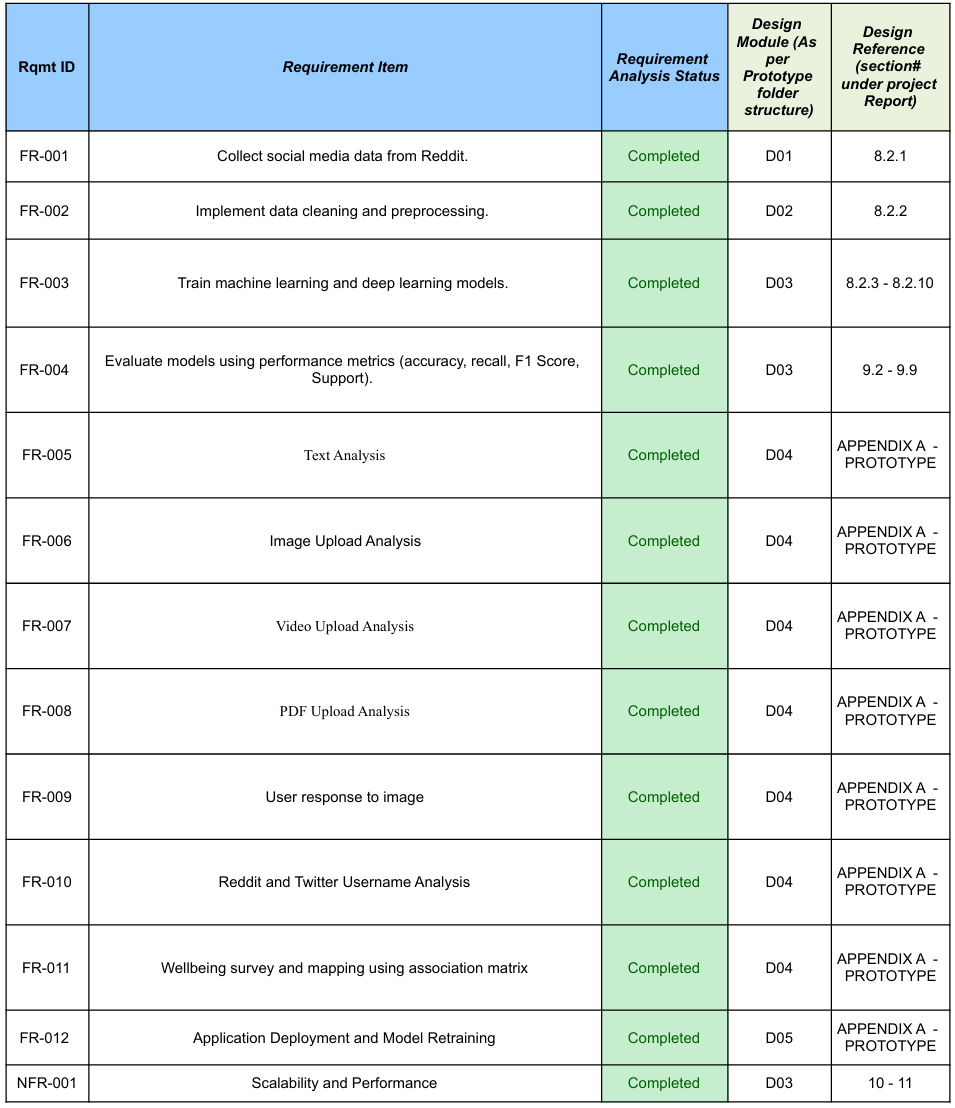
\includegraphics[width=1.0\textwidth]{Images/Requirement Matrix.png}  
    \caption{Requirement Matrix}
    \label{Requirement Matrix}  % Label for referencing the figure
\end{figure}

\noindent
The Requirement Matrix is a comprehensive tool used to track and manage the key requirements of a project. It systematically organizes each requirement with a unique identifier, description, priority, and category (such as functional or non-functional). The matrix also records the source of the requirement, its current status (e.g., in progress, completed), any dependencies on other requirements, and the team or individual responsible for fulfilling it. Additionally, it includes a verification method to ensure the requirement is met, such as through testing or review. This structured format helps ensure that all requirements are clearly defined, prioritized, and tracked, enabling effective project management and ensuring alignment with stakeholder expectations.

\subsection{Requirement Elaboration}
% Create separate sections for separate areas of requirement as in Requirement Matrix. 
% \vspace{.1in}

% \noindent
% For \textbf{Requirement Elaboration}, titles of s6.2.1, 6.2.2 etc. should be with the name of respective requirement areas. Your focus should be on: “What is needed in the system?” Requirement IDs should match with the ID column under Requirement Matrix.

\subsubsection{Functional Requirements}

\noindent
\textbf{\emph{Requirement ID: FR-001}} \\ 
\textbf{\emph{Description: Data Collection}} \\
\textbf{\emph{Priority: High}} \\
\textbf{\emph{Category: Functional}} \\
\noindent
The system requires an ability to collect and ingest a large dataset of Reddit posts using Python Reddit API Wrapper. The data should include text content from tweets, associated sentiment labels, and other metadata such as timestamp and user details. This will serve as the primary source of information for mental health disorder detection. The system must ensure that the dataset is loaded correctly into the machine learning environment, and any discrepancies in the structure should be handled with pre-processing steps like cleaning, normalization. \\

\noindent
\textbf{\emph{Requirement ID: FR-002}} \\ 
\textbf{\emph{Description: Data Cleaning and Preprocessing}} \\
\textbf{\emph{Priority: High}} \\
\textbf{\emph{Category: Functional}} \\
\noindent
The system must include modules to clean the raw data, such as removing irrelevant characters, handling missing data, and tokenizing text. For the social media posts, it is essential to remove URLs, stopwords, and unnecessary punctuation. The pre-processing pipeline should also convert the text into a suitable numerical format using Term Frequency-Inverse Document Frequency (TF-IDF) for further analysis. Proper pre-processing ensures that the data is in a form that can be efficiently used by machine learning models. \\

\noindent
\textbf{\emph{Requirement ID: FR-003}} \\ 
\textbf{\emph{Description: Training Machine and Deep Learning Models}} \\
\textbf{\emph{Priority: High}} \\
\textbf{\emph{Category: Functional}} \\
\noindent
The system needs to implement machine learning algorithms such as Logistic Regression and XGboost to classify social media posts based on text and detect potential signs of mental health disorders. The system must be able to train these models on historical data and then apply them to predict the sentiment and detect mental health-related issues in new posts. \\

\noindent
\textbf{\emph{Requirement ID: FR-004}} \\ 
\textbf{\emph{Description: Model Validation and Evaluation}} \\
\textbf{\emph{Priority: High}} \\
\textbf{\emph{Category: Functional}} \\
\noindent
The system must evaluate the performance of the trained models by splitting the dataset into training and test sets. Various performance metrics like accuracy, precision, recall, and F1-score should be computed to assess the model’s effectiveness in detecting mental health disorders. Based on the evaluation, the system should allow for model fine-tuning, such as adjusting hyperparameters, to improve the overall performance. 


\subsubsection{Non Functional Requirements}

\noindent
\textbf{\emph{Requirement ID: NFR-001}} \\ 
\textbf{\emph{Description: Testing}} \\
\textbf{\emph{Priority: Medium}} \\
\textbf{\emph{Category: Non Functional}} \\
\noindent
The addition of testing as a non-functional requirement ensures that the system is not only usable in the short term but also maintainable and extensible over time. This guarantees that future updates and improvements to the system can be implemented without disrupting existing functionality or requiring a steep learning curve for new developers or users. \\

\noindent
\textbf{\emph{Requirement ID: NFR-002}} \\ 
\textbf{\emph{Description:  Deployment}} \\
\textbf{\emph{Priority: Medium}} \\
\textbf{\emph{Category: Non Functional}} \\
\noindent
The system must be deployed considering the potential growth in the amount of social media posts that need to be analyzed. The data processing pipeline should be scalable to handle increasing data size without significant degradation in performance. This could involve implementing parallel processing techniques or leveraging cloud-based infrastructure to ensure that processing large datasets remains feasible even as the dataset scales. 

\vspace{1em}
\noindent
The system is designed to support comprehensive mental health disorder detection from social media posts, with key functional and non-functional requirements. It requires the ability to collect and ingest large datasets of Reddit posts using the Python Reddit API Wrapper, capturing text content, sentiment labels, timestamps, and user metadata. This data forms the foundation for analysis, necessitating robust pre-processing steps to ensure quality and consistency. The pre-processing pipeline must clean raw data by removing irrelevant characters, URLs, and stopwords, handling missing values, and tokenizing text. Additionally, text should be converted into numerical formats using techniques like Term Frequency-Inverse Document Frequency (TF-IDF) for model training. The system incorporates machine learning algorithms such as Logistic Regression and XGBoost to classify social media posts and detect potential mental health disorders. It must support training these models on historical data while applying them to predict and classify new posts. To ensure model reliability, the system splits data into training and test sets, evaluating performance using metrics like accuracy, precision, recall, and F1-score. Model fine-tuning, including hyperparameter adjustments, is essential for optimizing performance. Non-functional requirements focus on testing to ensure the system remains maintainable and extensible, enabling future updates without significant disruption. Additionally, deployment considerations emphasize scalability to process increasing volumes of social media posts, leveraging parallel processing and cloud infrastructure to maintain efficiency. Together, these requirements provide a robust framework for effective and scalable mental health detection.

% -------------------- Requirement Analysis Ends -----------------------------
